%% ==============================
\chapter{\iflanguage{ngerman}{Ergebnisse}{Results}}
\label{sec:results}
%% ==============================





Diese Kapitel beschäftigt sich mit den Ergebnissen und der Evaluation dieser Bachelorarbeit. Die Ergebnisse der Visualisierung sind in mehreren Abbildungen zu sehen. Die Evaluation teilt sich folgendermaßen auf. Als erstes werden die Ergebnisse der Visualisierung des Ventrikelsystems gezeigt und evaluiert. Dabei wurde für die Auswertung ein Interview mit einem Arzt durchgeführt. Danach wird eine Nutzerstudie vorgestellt, die die Benutzerfreundlichkeit des Systems testet. Als letztes wird die Berechnungszeit der Implementierung besprochen.


\subsection{Visualisierung}

\todo{formulierung}
Die in diesem Unterkapitel gezeigten Visualisierungen wurde alle auf Volumen mit einer Auflösung von 256x101x256 Pixeln berechnet. Aus dem Grund, dass diese ein gute Balance zwischen der Auflösung und der Berechnungszeit darstellt. Im Unterkapitel  Berechnungszeiten wird dies genauer beschrieben. Bevor die Visualisierung ausgewertet werden kann, wird zunächst das Ventrikelsystem erläutert.
\newline
In \autoref{fig:ventrik} ist das Ventrikelsystem zu sehen. Dieses besteht aus vier verschiedenen Ventrikeln. Zum einen der linke und der rechte Seitenventrikel, oberen beiden Bögen, die in der Abbildung zu sehen sind. Zum anderen der dritte und vierte Ventrikel, die zwischen den beiden Seitenventrikeln liegen und nach unten weggehen. Die Seitenventrikel bestehen aus einem Vorderhorn, Nr. 1,  einem Hinterhorn, Nr. 2, und einem Unterhorn, Nr. 3. Der dritte Ventrikel ist mit der Nummer 4 und der vierte Ventrikel mit der Nummer 5 versehen.
\newline
Bei der Ventrikelpunktion, wird einer der beiden Seitenventrikel im vorderen Bereich punktiert. Dies macht vor allem die Darstellung der Seitenventrikel relevant.

\begin{figure}[!h] 
\centering 
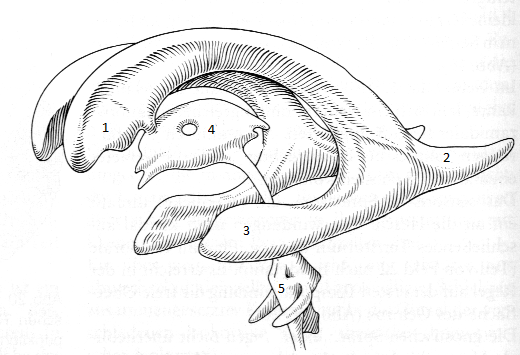
\includegraphics[width=0.75\textwidth]{Logos/Ventrikelsystem_V.png}
\caption{Ventrikelsystem} 
\label{fig:ventrik} 
\end{figure}
\todo{richtiges bild finden, quelle angeben}



Das Verfahren wurde an 15 verschiedenen CT-Datensätzen von der Uni Ulm getestet. Darunter waren verschiedene Ventrikelsysteme. Vier der Datensätze waren von Menschen mit einem normalen Ventrikelsystem, vier andere wiesen ein sehr schlankes System auf. Weiterhin litten zwei Patienten unter Atrophie, einem, oft durch das Alter verursachtem, Schwund an Gehirnmasse. Zwei andere Datensätze waren von Leuten, die unter einem Mittellinienshift litten. Dies bezeichnet die Verschiebung der Mittellinie der Ventrikelsystems, was beispielsweise durch einen Schlag auf den Kopf hervorgerufen werden kann. Weiterhin gab es Daten, von einer Hirnblutung, und einem Hydrocephalus, einer Aufstauung von Nervenwasser im Kopf. Als letztes gab es noch Daten eines deformierten Ventrikelsystems, ausgelöst durch Wassereinlagerungen im Gehirn.
\newline
Eine erfolgreiche Visualisierung gelang in nur 3 der 15 Fälle und zwar bei zwei Datensätzen mit normalen Ventrikeln und einem von einem Patient, der unter Atrophie leidet. In \autoref{fig:norm1_s} und \autoref{fig:norm1_u} ist die Visualisierung des ersten normalen Ventrikelsystems, in \autoref{fig:norm2_s} und \autoref{fig:norm2_u} die Visualisierung des zweiten normalen Ventrikelsystems und schließlich in \autoref{fig:atro_s} und \autoref{fig:atro_u} die Visualisierung des Ventrikelsystems des Patienten mit Atrophie zu sehen. Die Abbildungen zeigen Screenshots aus der Darstellung in Unity, jeweils aus den Perspektiven von der Seite und von oben.

\begin{minipage}[c]{0.49\textwidth}
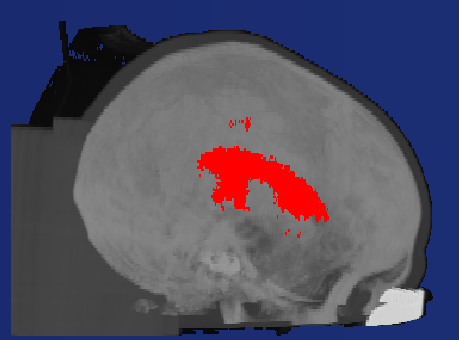
\includegraphics[width=\textwidth]{Logos/Normal1/Seite.PNG}
\captionof{figure}{Visualisierung des ersten normalen Ventrikelsystems von der Seite}
\label{fig:norm1_s}
\end{minipage}
\begin{minipage}[c]{0.49\textwidth}

\includegraphics[width=\textwidth]{Logos/Normal1/Unten.PNG}
\captionof{figure}{Visualisierung des ersten normalen Ventrikelsystems von Unten}
\label{fig:norm1_u}
\end{minipage}


In \autoref{fig:norm1_s}, der Darstellung des ersten normalen Ventrikelsystems von der Seite, sind links über dem Hinterhorn der Seitenventrikel Punkte zu erkennen, die nicht zum Ventrikelsystem gehören. Auch bei den Visualisierungen der andern Ventrikelsysteme sind an mehreren Stellen solche Ausreißer zu erkennen. Diese können bei dem aktuellen Stand der Implementierung nicht entfernt werden und senken die Qualität der Darstellung. 



\begin{minipage}[c]{0.49\textwidth}
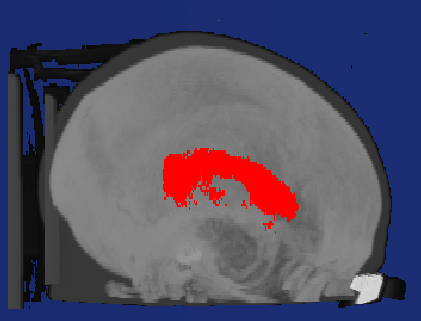
\includegraphics[width=\textwidth]{Logos/Normal2/Seite.PNG}
\captionof{figure}{Visualisierung des zweiten normalen Ventrikelsystems von der Seite}
\label{fig:norm2_s}
\end{minipage}
\begin{minipage}[c]{0.49\textwidth}

\includegraphics[width=\textwidth]{Logos/Normal2/Unten.PNG}
\captionof{figure}{Visualisierung des zweiten normalen Ventrikelsystems von Unten}
\label{fig:norm2_u}
\end{minipage}



\begin{minipage}[c]{0.49\textwidth}
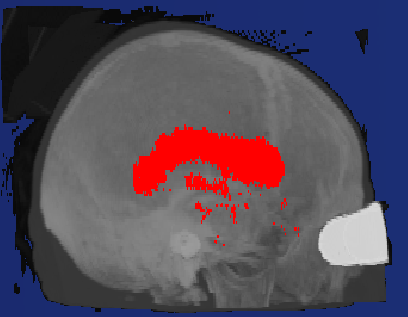
\includegraphics[width=\textwidth]{Logos/Atrophie/Seite.PNG}
\captionof{figure}{Visualisierung des Atrophie Ventrikelsystems von der Seite}
\label{fig:atro_s}
\end{minipage}
\begin{minipage}[c]{0.49\textwidth}

\includegraphics[width=\textwidth]{Logos/Atrophie/Unten.PNG}
\captionof{figure}{Visualisierung des Atrophie Ventrikelsystems von Unten}
\label{fig:atro_u}
\end{minipage}




Für die drei erfolgreich visualisierten Daten wurde zur Evaluation ein Arzt von der Uniklinik Ulm interviewt. Diesem wurden die Visualisierungen direkt in Unity vorgeführt. Während der Vorführung konnte der Mediziner selbst die Kamera durch die Darstellung lenken und das Ergebnis aus verschiedenen Blickwinkeln betrachten. Anschließend bewertete er die Qualität der Ergebnisse, indem er drei verschiedenen Fragen zu den Darstellungen beantwortete. Er musste dabei seine Antwort immer auf einer Skala von 1 bis 5 angeben.
\newline
Die Fragen lauteten:
\begin{itemize}
	\item 1) Wie gut ist das Ventrikelsystem bei der Visualisierung zu erkennen? \newline sehr schlecht 1 - 5 sehr gut
	\item 2) Wird das Ventrikelsystem in der Visualisierung vollständig dargestellt? \newline überhaupt nicht vollständig 1 - 5 vollständig
	\item 3) Wie genau ist das Ventrikelsystem segmentiert? \newline überhaupt nicht segmentiert 1 - 5 ausschließlich das Ventrikelsystem ist segmentiert
\end{itemize}


Die Ergebnisse der Antworten des Arztes werden in \autoref{tab:ergebnis_arzt} gezeigt. Allgemein merkte der Mediziner jedoch an, dass bei jeder Visualisierung, die durch das Verfahren erzeugt wurde, nur der linke und rechte Seitenventrikel zu sehen war. Die deutlich schmaleren dritten und vierten Ventrikel und die Unterhörner der Seitenventrikel fehlten bei den Darstellungen komplett. Er erklärte jedoch, dass diese bei einem gesunden Menschen jedoch sehr dünn und deshalb anhand von CT-Daten schwer zu segmentieren seien. Weiterhin sind, wie schon erwähnt, die Seitenventrikel entscheidend für eine erfolgreiche Punktion. In folge dessen, wurde sich darauf geeinigt, dass die Beantwortung der zweiten Frage, nach der Vollständigkeit des Ventrikelsystems, lediglich auf die Vollständigkeit der beiden Seitenventrikel bezogen ist.

\begin{table}[h]
\centering
\resizebox{\columnwidth}{!}{
 \begin{tabular}{| c | c | c | c |}
  \hline
  Ventrikelsystem & 1. Frage & 2.Frage & 3. Frage\\ \hline
  Normal 1 & 4 & 4 & 3 \\ \hline
  Normal 2 & 4 & 2 & 3\\ \hline
  Atrophie & 4 & 3 & 2 \\ \hline
 \end{tabular}
 }
\caption{Ergebnisse des Interviews mit einem Arzt}
\label{tab:ergebnis_arzt}
\end{table}


Die Bewertung des ersten normalen Ventrikelsystems fiel positiv mit 11 von möglichen 15 Punkten aus. Das Ventrikelsystem war als solches klar und deutlich zu erkennen, jedoch fehlte ein Teil der Hinterhörner. Bis auf diese waren die Seitenventrikel jedoch vollständig zu sehen. Weiterhin war die Segmentierung nicht exakt, da es mehrere kleine Ausreißer gab.
\newline
Das zweite normale Ventrikelsystem, war ebenfalls klar zu erkennen. Jedoch wurde fast ausschließlich der linke Seitenventrikel segmentiert. Die Bewertung der Vollständigkeit fiel mit einer vier so hoch aus, da der eine Seitenventrikel sehr klar, deutlich und vollständig zu sehen war. Der Arzt sagte, dass dieser besser und glatter als die des ersten normalen Ventrikelsystems sein, da man auch das Hinterhorn erkennen kann. 
\newline
In einem Gehirn eines unter Atrophie leidenden Menschen, ist deutlich mehr Liquor, als bei einem gesunden Menschen, zu finden. Diese Flüssigkeiten werden vom Verfahren ebenfalls erkannt, weshalb die Segmentierung etwas verschwommen erscheint und nicht die kompletten Seitenventrikel erfasst werden. Jedoch vermutete der Arzt, dass viele der Ausreißer zum dritten Ventrikel gehören, da sich dieses, wie alle Ventrikel bei einer Atrophie, weitet. Trotz der Flüssigkeiten im Gehirn war das Ventrikelsystem in der Darstellung deutlich zu erkennen.
\newline
 Im Allgemeinen sagte der Mediziner, dass das Ventrikelsystem bei allen Visualisierungen als solches eindeutig zu erkennen sei. Er bemängelte jedoch, dass die Darstellungen nicht glatt genug sei und zu viele Ausreißer besitzen.




Zur weiteren Auswertung der Ergebnisse wurde das erste normale Ventrikelsystem aus \autoref{fig:norm1_s} und \autoref{fig:norm1_u} in Unity und mit der MITK-Workbench, die auch zum Umwandeln der DICOM-Dateien benutzt wurde, visualisiert.
\newline
In Unity wurde dabei die Erweiterung zum hervorheben von Wertebereichen benutzt. Diese wurde auf 1025 bis 1030 eingestellt, da das Ventrikelsystem Intensitätswerte in diesem Bereich hat. Die Ergebnisse sind in \autoref{fig:unity_s} und \autoref{fig:unity_u} zu sehen.
\newline
Das Ventrikelsystem ist zwar zu sehen, es gibt jedoch sehr viele Ausreißer, die es fast unmöglich machen die Ventrikel zu erkennen. Diese simple Vorgehensweise führt zu keinem gewünschtem Ergebnis.
\newline
In der MITK-Workbench gibt es verschiedene Segmentierungstools. Darunter ist ein Region Growing Tool, bei dem der Nutzer einen \textit{seed} Punkt in den Schnittbildern wählen kann. Über die verwendete Kostenfunktion werden keine Informationen genannt. Anschließend können die Löcher der Auswahl mit einem \textit{closing} Filter geschlossen und mit einem weiteren Tool ein geglättete 3D Ansicht des Ergebnis erzeugt werden. Screenshots des Ergebnisses sind in \autoref{fig:mitk_o} und \autoref{fig:mitk_v} zu sehen.
\newline
In dem von der Workbench erzeugte Ergebnis ist das Ventrikelsystem gut zu erkennen. Die Seitenventrikel sind vollständig und besitzen eine glatte Oberfläche. Sogar große Teile des dritten und vierten Ventrikels sind teil der Segmentierung. Allerdings sind auch ganze Bereiche hervorgehoben, die nicht zum Ventrikelsystem gehören. Diese könnten vom Benutzer manuell in jedem Schichtbild des Datensatzes entfernt werden, was jedoch sehr zeitaufwändig wäre.
\todo{drüber schauen}


\begin{minipage}[c]{0.49\textwidth}
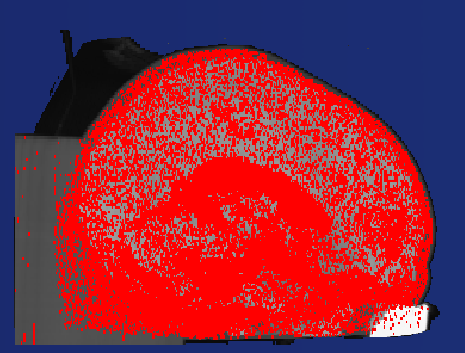
\includegraphics[width=\textwidth]{Logos/Normal1_Unity/Seite.PNG}
\captionof{figure}{Visualisierung des ersten normalen Ventrikelsystems von der Seite mithilfe von Unity}
\label{fig:unity_s}
\end{minipage}
\begin{minipage}[c]{0.49\textwidth}

\includegraphics[width=\textwidth]{Logos/Normal1_Unity/Unten.PNG}
\captionof{figure}{Visualisierung des zweiten normalen Ventrikelsystems von Unten mithilfe von Unity}
\label{fig:unity_u}
\end{minipage}


\begin{minipage}[c]{0.49\textwidth}

\includegraphics[width=\textwidth]{Logos/Normal1_MITK/Oben.PNG}
\captionof{figure}{Visualisierung des ersten normalen Ventrikelsystems von Oben mithilfe von MITK}
\label{fig:mitk_o}
\end{minipage}
\begin{minipage}[c]{0.49\textwidth}
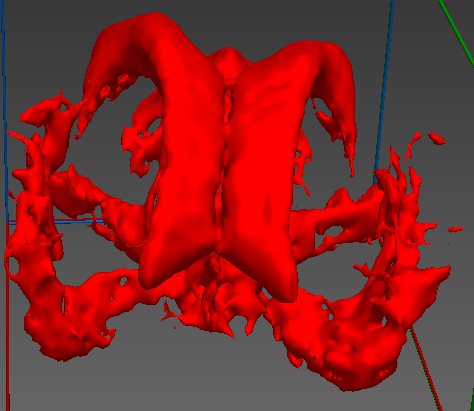
\includegraphics[width=\textwidth]{Logos/Normal1_MITK/Schraeg_Vorne.PNG}
\captionof{figure}{Visualisierung des ersten normalen Ventrikelsystems von Vorne mithilfe von MITK}
\label{fig:mitk_v}
\end{minipage}


\subsection{Nutzerstudie}


\todo{nutzerstudie variablen etc. erwähnen -> proseminar}
\todo{info über teilnehmer}
Im Rahmen der Evaluation der Benutzerfreundlichkeit des Verfahrens wurde eine kleine Nutzerstudie mit ... Teilnehmern durchgeführt. Bei dieser wurden den Probanden zunächst der Ablauf und die vom Benutzer erforderlichen Schritte um eine Visualisierung des Ventrikelsystems zu erhalten durch eine Vorführung durch den Interviewer gezeigt. Anschließend mussten die Teilnehmer selbst das eben gelernte anwenden und das Programm selber ausführen. Dabei bekamen sie, wenn sie nicht weiterwussten, Hilfe vom Versuchsleiter. Als Abschluss füllten die Probanden einen NASA-TLX Bogen zu der Aufgabe aus. Die durchschnittlichen Ergebnisse der einzelnen Kategorien wird in \autoref{tab:ergebnis_nasa} gezeigt.


\begin{table}[h]
\centering
\resizebox{\columnwidth}{!}{
 \begin{tabular}{| c | c | c | c |}
  \hline
  Kategorie & Gewichtung & Klicks & Wichtung \\ \hline
  Geistige Anforderung & 0&0 &0 \\ \hline
  Körperliche Anforderung & 0& 0& 0\\ \hline
  Zeitliche Anforderung &0 &0 &0 \\ \hline
  Leistung &0 &0 & 0\\ \hline
  Anstrengung &0 & 0& 0\\ \hline
  Frustration &0 &0 & 0\\ \hline 
 \end{tabular}
 }
\caption{Durchschnittlichen Ergebnisse des NASA-TLX Bogens}
\label{tab:ergebnis_nasa}
\end{table}


Der durchschnittliche Wert für die Gesamtbeanspruchung lag bei ... Personen ohne Programmiererfahrung ...

 
Trotz der Schwierigkeiten,  gaben die Probanden an, dass sie die Aufgabe mit einer guten ausführlichen Dokumentation auch alleine ohne Hilfe hinbekommen würden.


\subsection{Berechnungszeit}

Die folgenden Zeitmessungen wurde alle auf einem Computer mit einem 3.70GHz  Intel Core(TM) i7-8700K CPU mit 32GB RAM ausgeführt.
\newline
Um die Berechnungszeit des Systems evaluieren zu können, wurde die Kalkulation des gesamten Clusteringverfahrens sowie die Berechnung des LH-Histogramms auf drei Volumen verschiedener Größen durchgeführt. Damit der Vergleich nicht von unterschiedlichen Volumendaten verfälscht wird, wurden alle Volumen aus dem gleichen CT-Datensatz generiert. Dabei wurde die Originalgröße mit einer Auflösung von 512x201x512 Pixeln mithilfe des Resamplemoduls des Helpers verkleinert. Die beiden anderen Volumengrößen haben dabei die  Hälfte, mit 256x101x256 Pixeln, und Dreiviertel, mit 384x151x384 Pixeln, der Auflösungen des Originalvolumens. Es war geplant, dass noch ein viertes Volumen zum Vergleich hinzugezogen wird.Jedoch war es aus einem unbekannten Fehler leider nicht möglich die beiden Berechnungen mit dem gevierteltem Originalvolumen durchzuführen. Des Weiteren funktioniert für beim Originalvolumen lediglich die Berechnung des LH-Histogramms. Die Kalkulation des Clusteringverfahrens war nicht möglich, vermutlich aus dem Grund, dass bei dieser hohen Auflösung es zu viele Daten für die aktuelle Implementierung zu berechnen gibt.
\newline
Die Berechnungszeit hängt stark von der Größe des Eingabevolumens ab. Die ist in \autoref{tab:ueberblick_zeit} sehr gut zu erkennen. Diese zeigt einen Überblick über die ungefähren Berechnungszeiten der verschiedenen Volumengrößen.


\begin{table}[h]
\centering
\resizebox{\columnwidth}{!}{
 \begin{tabular}{| c | c | c | c |}
  \hline
  Volumengröße & LH-Histogramm $[s]$ & Komplettes Verfahren $[s]$ \\ \hline
  Halbes Volumen (256x101x256)  & 30 &  50	\\ \hline
  Dreiviertel Volumen (384x151x384)  & 90 &  380	\\ \hline
  Ganzes Volumen (512x201x512) & 225 & -	\\ \hline
 \end{tabular}
 }
\caption{Überblick über die Berechnungszeiten der verschiedenen Volumengrößen}
\label{tab:ueberblick_zeit}
\end{table}


Dabei ist wichtig zu beachten, dass die Zeit zur Berechnung der LH-Histogramme die gleiche Zeit wie die Kalkulation der LH-Werte im gesamten Verfahren benötigt. Die Berechnungsdauer der Gradienten ist hierbei zirka doppelt so lange wie die der LH-Werte. Wird die Berechnungszeit des Histogramms von der Kalkulationszeit des gesamten Verfahrens abgezogen, kommt die Zeit, die die beiden Clusteringschritte benötigen heraus.
\newline
Eine interessante Beobachtung hierbei ist, dass die Berechnung der LH-Histogramme abhängig von der Anzahl der Pixel gesehen in etwa gleich schnell abläuft. Das halbe Volumen hat eine Gesamtpixelzahl von ungefähr 6,6 Millionen, das dreiviertel Volumen von zirka 22,2 Millionen und das Original von grob 52,6 Millionen Pixeln. Wird die Anzahl an Pixeln die pro Sekunde bei der LH-Wert Berechnung bearbeitet werden für diese drei Volumen berechnet, so ist zu beobachten, dass keine großen Unterschied zwischen den Zeiten existiert. Das Halbe bearbeitet etwa 220 Tausend, das Dreiviertel ungefähr 247 Tausend und das Ganze 234 Tausend Pixel pro Sekunde. Der kleine Unterschied in der Rate lässt sich einerseits durch Volumen unabhängige Berechnungen, und andererseits durch Messfehler erklären. Folglich kann man sagen, dass die Berechnungszeit der LH-Werte bei dieser Implementierung in etwa linear mit der Anzahl an Eingabepixeln wächst.
\newline
Auf der anderen Seite ist jedoch auch zu erkennen, dass die beiden Clusteringschritte mit zunehmender Eingabegröße deutlich langsamer werden. Das Clustering des halben Volumens dauerte 20 Sekunden und hat damit eine Verarbeitungsrate von zirka 330 Tausend Pixeln pro Sekunde. Hingegen dauert es beim dreiviertel Volumen 290 Sekunden und erreicht damit gerade einmal einen Rate von 76 Tausend Pixeln pro Sekunde. Es benötigt also 14,5 mal so viel Zeit für die 3,3 fache Anzahl an Pixeln.














































